\documentclass{article}
\usepackage[utf8]{inputenc}
\usepackage{graphicx}
\usepackage{titlepic}
\usepackage{caption}
\usepackage{subcaption}
% \documentclass{beamer}

\newcommand{\namesigdate}[2][5cm]{%
  \begin{tabular}{@{}p{#1}@{}}
    #2 \\[0.4\normalbaselineskip] \hrule \\[0pt]
    {\small } \\[2\normalbaselineskip] 
  \end{tabular}
}

\title{\vspace*{\fill} \textbf{Video Description using Deep Learning}
	  \\ {\large \textbf{Summer Undergraduate Research Award}}
	  \\  \vspace{3mm} 
\includegraphics[width=5cm]{logo.png}}

\author{
	\textbf{Suyash Agrawal}\\ 
	2015CS10262\\
	Computer Science\\
	CGPA: 9.91 \\
	Mob: 9717060183\\
	cs1150262@iitd.ac.in
	\and
	\textbf{Madhur Singhal}\\ 
	2015CS10235\\
	Computer Science\\
	CGPA: 8.66\\
	Mob: 9540972599\\
	cs1150235@iitd.ac.in
}
\date{\textbf{Supervisor:-} \\ \textbf{Subhashis Banerjee} \\ Professor \\ Department of CSE \\ suban@cse.iitd.ac.in\\ IIT Delhi\\
\vspace*{\fill}}




\begin{document}
		% 
\includegraphics{logo.png}
	\maketitle

% \noindent \namesigdate{} \hfill \namesigdate[3cm]{Saroj Kaushik \\ HOD CSE }
% \begin{flushleft}
% \noindent \namesigdate{} 
% \end{flushleft}

\begin{center}
\noindent\rule{3.2cm}{0.4pt} 
\end{center}

\begin{flushright}
\noindent\rule{3.2cm}{0.4pt} 
\\ \textbf{Prof. S. Arun Kumar}
\\ Head of Department
\\ Department of CSE
\\ sak@cse.iitd.ernet.in
\end{flushright}


	\newpage
	% \begin{figure}
% \end{figure}
	
	\section{Introduction}
		\textit{\textbf{Video Description}} is the process of discovering knowledge, structures, patterns and events of interest in the video data and describing them in natural language. Video Description is an incredibly hard problem in computer vision and currently the only source of video description is manual labour. 
		\newline
		Video Description has wide variety of applications. It can help visually impared people "see" the world by describing the scene around them. It has also use in automated survelliance by analysing the videos in real time and reporting criminal activites. Also, it can be used to efficiently index large video databases based upon their content for ease of accessibility.

		\begin{figure}[ht!]
		\centering
		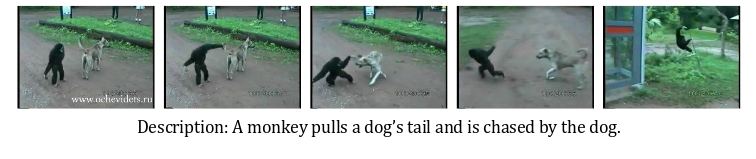
\includegraphics[width=12.5cm]{description.png}
		\caption{Sample Video Description\label{fig}}
		\end{figure}		
		
%		\begin{figure}[ht!]
%			\centering
%			\begin{subfigure}{.5\textwidth}
%			  	\centering
%			  	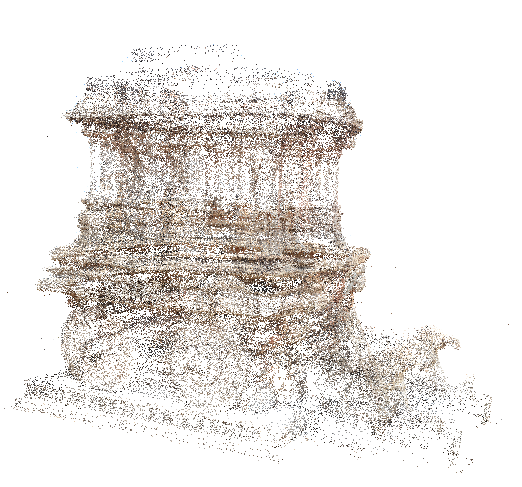
\includegraphics[width=1.0\linewidth]{sparse_chariot.png}
%			  	\caption{Sparse reconstruction}
%			  	\label{fig:sub1}
%			\end{subfigure}%
%			\begin{subfigure}{.5\textwidth}
%			  	\centering
%			  	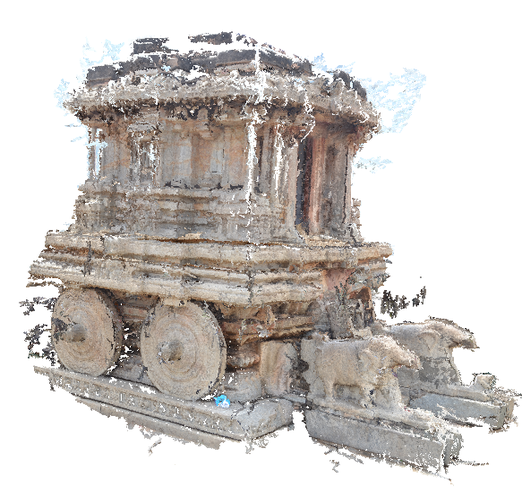
\includegraphics[width=1.0\linewidth]{dense_chariot.png}
%			  	\caption{Dense reconstruction}
%			  	\label{fig:sub2}
%			\end{subfigure}
%			\caption{3D reconstruction}
%			\label{figstart}
%		\end{figure}


		Figure~\ref{fig:fig0} shows a possible description of a sample video. The \textit{traditional pipeline} is shown in Figure~\ref{fig3}.

		\begin{figure}[ht!]
		\centering
		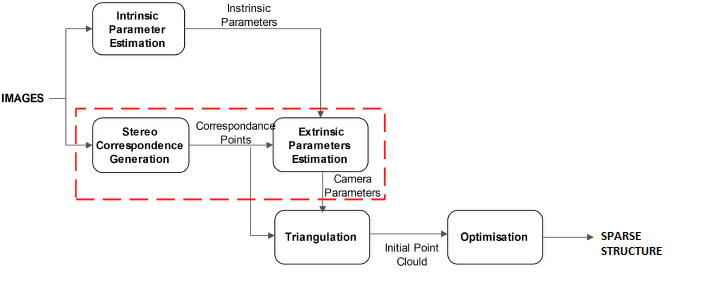
\includegraphics[width=14cm]{traditional_pipeline2.png}
		\caption{Traditional pipeline\label{fig3}}
		\end{figure}

		The red-highlighted part of the pipeline is \textit{\textbf{computationally expensive}}. Thus, our project aims to reduce this computation and perform 3D reconstruction in near real-time.

		The processing parts are:
			\begin{itemize}
			\item \textit{Intrinsic and extrinsic parameters}: The camera projection matrix is a $3 \times 4$ matrix which represents the pinhole geometry of a camera for mapping 3D points in the world coordinates to 2D points on images. This matrix depends on extrinsic and intrinsic parameters. The intrinsic parameters mainly comprises of focal length, image sensor format, and principal points. The extrinsic parameters define the position of the camera center and the camera's heading in world coordinates in terms of a rigid rotation and translation. 
			\item \textit{Stereo correspondence generation}: Given two or more images of the same 3D scene, taken from different points of view, the correspondence problem refers to the task of finding a set of points in one image which can be identified as the same points in another image. To do this, points or features in one image are matched with the corresponding points or features in another image. The images can be taken from a different point of view, at different times, or with objects in the scene in general motion relative to the camera(s).
			\item \textit{Triangulation}: Triangulation refers to the process of determining a point in 3D space given, its projections onto two or more images and their corresponding camera projection matrices. This point is found as the intersection of the two or more projection rays formed from the inverse projection of the 2D image points representing that 3D point in space.
			\item \textit{Initial point cloud and 3D sparse reconstruction}: As the word suggests, \textit{3D sparse construction} is done for only some set of data points in the given coordinate system called \textit{initial point cloud}. Figure~\ref{fig:sub1} illustrates a 3D sparse construction of a chariot. Figure~\ref{fig:sub2} illustrates 3D dense construction of the same initial point cloud.

			\end{itemize}
	\section{Objectives} 
		Our main objective is to perform 3D reconstruction in near real time using a mobile device. This can be further be subdivided into following points:
		\begin{enumerate}
			\item 
				To get accurate position and orientation estimate based on readings of IMU sensors in smart-phones. 
			\item
				To use the camera feed in smart-phones to enhance the position estimate based on visual tracking of objects.
			\item 
				To do sparse 3D reconstruction based on sensor fusion data and computer vision techniques.
			\item
				To enhance the quality and efficiency of 3D reconstruction by adding more details and moving towards dense 3D reconstruction.
			\item
				We will ultimately be fusing digital signal processing and computer vision based techniques that will enable us to perform near real time 3D reconstructions on mobile or hand-held devices.
		\end{enumerate}

\section{Basic Concepts} 
		%\begin{itemize}
			\subsection{Convolutional Neural Networks}
			


			\subsection{Long Short Term Memory Networks}
			


			\subsection{Training Data}
			


			\subsection{Finetuning}
			

			\subsection{}




			\subsection{Camera calibration}
				The camera parameters can further be subdivided into intrinsic and extrinsic parameters. \textbf{Camera intrinsic parameter} $K$ is dependent on the focal length of the camera and principal point (which in most cases is the center of the image). The \textbf{camera extrinsic parameter} is composed of the rotation $R$ and translation $t$ between camera coordinate system and the world coordinate system. Together they form the camera projection matrix $P$, a $3 \times 4$ matrix which describes the mapping of a pinhole camera from 3D points in the world to 2D points in an image.
				\begin{equation}
				P = K[R|t]
				\end{equation}
			
			\subsection{Sparse 3D reconstruction} 
				Given two different images of the same scene from different angles, the position of a 3D point can be found as the intersection of the two projection rays which is commonly referred to as \textbf{triangulation}. For this first point correspondences have to be established. Then using this point correspondences a Random Sampling Consensus (RANSAC) based voting framework is used to estimate the camera intrinsic and extrinsic parameters. Finally, a joint non-linear optimization is used to further refine the camera parameters and the 3D points in a \textbf{bundle adjustment} framework. This method is computationally very expensive and hence done only for very sparse set of points. This is known as sparse 3D reconstruction.

			\section{Mobile IMU sensors}
				IMU (Inertial Measurement Unit) sensors are on-chip devices embedded in most of the smart phones or hand-held devices today. It mainly consists of a series of motion sensors: accelerometer, gyroscope, magnetometer and gravitation sensor. The data from these sensors can be fused to obtain the orientation and the position of the device in the world coordinate system.

			\section{Conventional versus mobile 3D reconstruction}
				In the case of a smart-phone or any hand-held device having a camera and IMU sensors, we wish to use  the IMU sensors to obtain extrinsic camera parameters in real time. This will help in reducing the load on conventional 3D reconstruction methods and get it in near real time.
		%\end{itemize}



	\section{Approach to the project} 
		First, we shall be using sensor fusion to obtain accurate estimates for camera position and orientation of the mobile device. Then we will move on to 3D reconstruction, which further has two parts: i.e. sparse 3D reconstruction and then use tracking to obtain dense correspondence of points for dense 3D reconstruction.
		\begin{enumerate}
			\item Position and orientation estimation
			\begin{enumerate}
				\item
					Get accelerometer data and orientation data at real time using the IMU sensors like accelerometer, gyroscope, gravity sensor and magnetometer present on the smart phone.
					This data is highly noisy. Figure~\ref{fig1} shows the position estimate from accelerometer data across various devices.

					\begin{figure}[ht!]
					\centering
					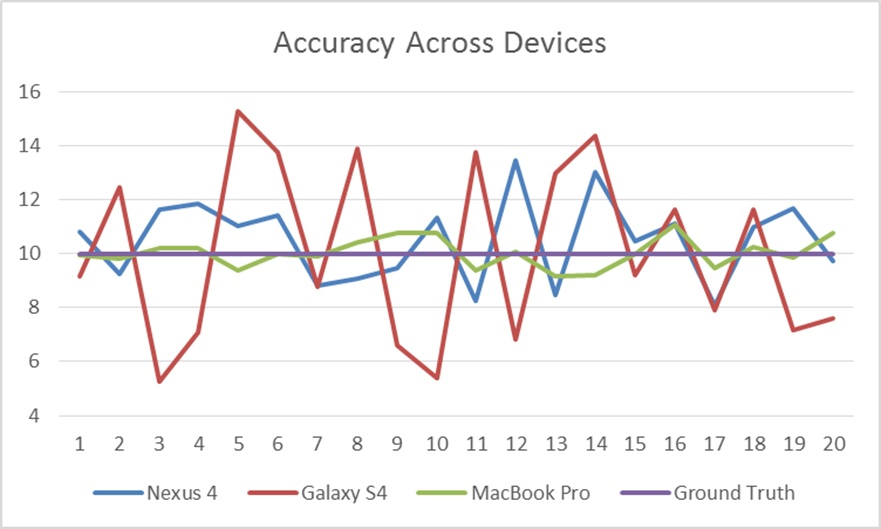
\includegraphics[width=10cm]{graph.jpg}
					\caption{Accuracy of accelerometer data across different devices (scale cm)\label{fig1}}
					\end{figure}

					As evident from the graph, this data cannot be directly used for calculation of position and orientation. 
					Figure~\ref{fig2} shows the integration of static accelerometer data to obtain velocity and displacement.

					\begin{figure}[ht!]
					\centering
					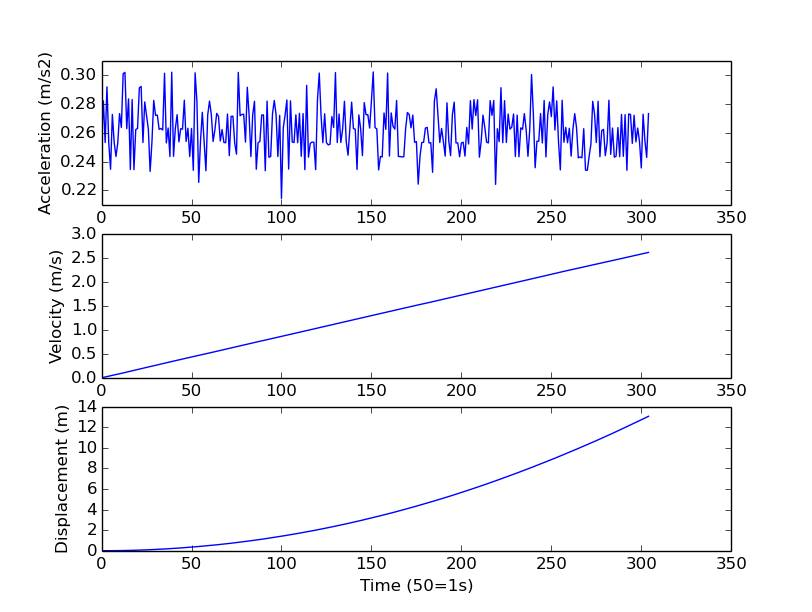
\includegraphics[width=10cm]{integration.jpg}
					\caption{Obtaining velocity and displacement from static accelerometer data\label{fig2}}
					\end{figure}

					The graph of both velocity and displacement shows significant deviation from the actual value which is zero.
					Thus, signal processing and smoothening is required to get a better estimate.

				\item
					Making the orientation data more accurate by infusing the higher frequency components from the gyroscope orientation after drift correction.
				\item
					Obtaining the displacement and orientation data from the camera feed on the device using visual tracking methods.
				\item
					A comparative study is to be done between the position estimates obtained by the two methods along with ground truth and fusing the results to obtain an enhanced position and orientation estimate.
			\end{enumerate}
			% • All these data along with the clicking of pictures are synchronised to a single system clock.
			% \item We will use the IMU sensors present in smart-phones to get a position estimation.
			\item 3D reconstruction
			\begin{enumerate}
				\item 
					Obtain sparse 3D reconstruction based on camera rotation and position parameters obtained previously.
				\item
					Use tracking data from different tracking methods like ``Good features to track'' or ``KL tracker'' for obtaining dense correspondence of points.
				\item
					Use guided matching by indirect computation of fundamental matrix from estimated camera motion from sensors to further enrich the correspondences.
				\item
					Triangulate the dense correspondences and do a final global refinement.					
			\end{enumerate}
			\item Further possibilities
			\begin{itemize}
			    \item Getting a more detailed texture mapping of the object.
			    \item Making an object recognition software on the basis of this 3D reconstruction.
			    \item Improving the algorithm for a quicker and more efficient 3D reconstruction. 
				\item Releasing applications for Apple, Android and Windows platforms for near real time 3D reconstruction on the device itself.
			\end{itemize}
		\end{enumerate}

	
	

	\section{Uses and applications}
	% \item Uses and Applications
			\begin{itemize}
				\item Using the device as an accurate measuring device. This can be of particular interest to blind as they will be able to measure distances and angles accurately with great ease.
				\item Doing real time dense 3D reconstructions on mobile phones and other hand-held devices. 
				\item Allowing the user to generate a 3D printable file on his mobile device. As 3D printers are becoming cheaper and more common, this feature will reduce the need of the person to use a 3D scanner to be able to generate prototypes of objects. This will allow engineers and students to work more efficiently as they can generate copies of 3D objects easily.
				\item This project can have applications in the field of archeology. It can be used to generate replica of artifacts and fragile objects for further studies, without harming its integrity.
				\item Our approach can also be applied in the field of medical sciences, especially for orthopedics and joint replacement surgery. The part to be replaced can be made with high accuracy using this project.
				\item The method can also be used by the astronauts up in space. With the help of our approach the parts to be changed can be easily made using a 3D printer.
				\item Localization at tourist sites and providing real time directions to landmark locations. This will involve the use of GPS (Global positioning system) as well to get a rough location of the user.
			\end{itemize}
	\newpage
	\section{Budget, duration and facilities}	
		\subsection{Budget}
			Rs. 25,000 will be needed to purchase an android smart phone having high quality sensors and a high resolution camera.
		\subsection{Duration}
			We will try to complete this project by the end of the summer break i.e. the end of July, 2015. 
		\subsection{Facilities}
		    \begin{itemize}
		    \item Access to the vision lab.
		    % \item Access to a computer in Vision Lab.
		    \end{itemize}
\end{document}